\documentclass[main.tex]{subfiles}


\begin{document}

\chapter{One-stage optimisation}\label{ch:onestage}

\todo[inline]{Write one-stage chapter}

The aim of this chapter is to discuss approaches to modelling a
decision problem in the form of a mathematical optimisation problem
that computer algorithms can solve.
We focus on one-stage optimisation problems here, which means that
we do not consider any temporal structure in the order of decisions.
The key concepts for defining an optimisation problem are~(i) a
collection of allowed decisions and~(ii) an ordering between all decisions.

If there is a deterministic relationship between allowed decisions
$x\in\mathcal{X}$ and one, well-defined, objective
$f:\mathcal{X}\to\mathbb{R}$, then we can model the decision problem
as the optimisation problem
\begin{equation}
  \min_{x\in\mathcal{X}} f(x).
\end{equation}
In this chapter, however, we will discuss three ways that
decision problems with random outcomes may deviate from this setting.
One, if there is a non-deterministic relationship between a decision
$x$ and outcomes of the system. Two, if we cannot
deterministically determine the allowed decisions
$\mathcal{X}$ at the time we make the decision. Three, if there are
multiple objectives.
We will argue that the second point arises when people try to add
non-determinism to a deterministic model without reconsidering the
modelling of the problem. One can view the first point as a decision
problem with a possibly infinite number of objectives.
\Cref{sec:one_optim_random_outcomes} summarises common ways to
model decision maker's that face non-deterministic outcomes modelled
with random variables, and \Cref{sec:one_multiobjective} summarises
the theory of multiobjective optimisation.

The ways to model an ordering between decisions have different
strengths and weaknesses. Often, the approaches that are appealing
from a theoretical point of view may be more expensive to compute and
approximate. There are situations where these methods can reach the
same decisions, with carefully adjusted parameters, as we show an
example of in \Cref{sec:one_comparison_orderings}. The take-home message from this chapter is
therefore to critically evaluate the complexity of the system we want
to control before formulating the mathematical optimisation problem.

\section{Optimisation with random outcomes}\label{sec:one_optim_random_outcomes}
In this section, we consider situations where there is one
well-defined objective that depends on  information we do not know
with certainty at the time we make the decision.

Define a decision-space $\mathcal{X}\subset \mathbb R^n$ and a
parameter-space $\mathcal{Y}\subset \mathbb R^k$.
Let $f:\mathcal{X}\times\mathcal{Y}\to\mathbb R$ be a twice continuously
differentiable function.
The aim is to choose $x\in\mathcal{X}$ in order to maximise $f$.
In the deterministic setting, we know the parameter
$y\in\mathcal{Y}$ and can therefore find the optimal $x$ by optimising
$f(\cdot,y)$.
Say there is uncertainty in the correct value of the parameter that
we model using an underlying probability distribution
on the Borel space of $\mathcal{Y}$, absolutely continuous with respect
to the Lebesgue measure.
For a given $x\in\mathcal{X}$, $f(x,\cdot)$ is now a random variable.
Thus, it is no longer straightforward to order two decisions $x_1$ and
$x_2$ by comparing $f(x_1,\cdot)$ to $f(x_2,\cdot)$.
We will present three classes of optimisation problems that attempt to
address the randomness of $f(x,\cdot)$. They are \emph{expected
  utilites}, \emph{mean-deviation procedures} and \emph{nonlinear
  expectations}.
At the end, we comment on classic optimisation problems with constraints
that are random variables.

\subsection{Expected utilities}
% Over all realisations of the parameter $y$, the average value of a
% choice $x\in\mathcal{X}$ is given by the expected value
% $\mathbb E[f(x,\cdot)]$. If the same optimisation is to be performed
% many times, and there is no danger of e.g.~bankruptcy, the choice that
% maximises expected value might be considered the optimal.
% In many problems, one only experiences one realisation of the
% parameter. For this realisation, the mean might not be a good
% representation of what a decision maker seeks.
One way to compare decisions in $\mathcal{X}$ is to consider a weighted
sum of all the realisations of the parameter in $\mathcal{Y}$.
Expected utilities weigh the different realisations by combining the
probability of an outcome with a measure of the benefit of $f$ for that
outcome.
A family of such measures of benefit are utility functions. The formal
theory of decisions that use expected utilities is covered in
\citep[Ch.~2]{follmer2004stochastic}.
\begin{mydef}[Utility function]
  A continuous function $u:\mathcal S\to\mathbb R$ on a set of outcomes
  $\mathcal S\subset \mathbb R$ defines a utility if
  it is increasing and concave.
  A \emph{risk-neutral} decision
  model is one where $u$ is linear, whilst a strictly concave utility function defines a
  \emph{risk-averse} decision model.
\end{mydef}

\begin{example}[Utility functions]
  Two popular utility functions are the exponential family
  $u_1(x)=1-e^{-\lambda x}$ with $\lambda>0$ and the logarithmic
  utility $u_2(x)=\log(1+x)$.
  The exponential utility is defined on $\mathcal S =\mathbb R$,
  whilst the logarithmic utility is only valid on $\mathcal
  S=[-1,\infty)$.
  \Cref{fig:example_utilities} shows behaviour near the origin.
  \begin{figure}[htbp]
    \centering
    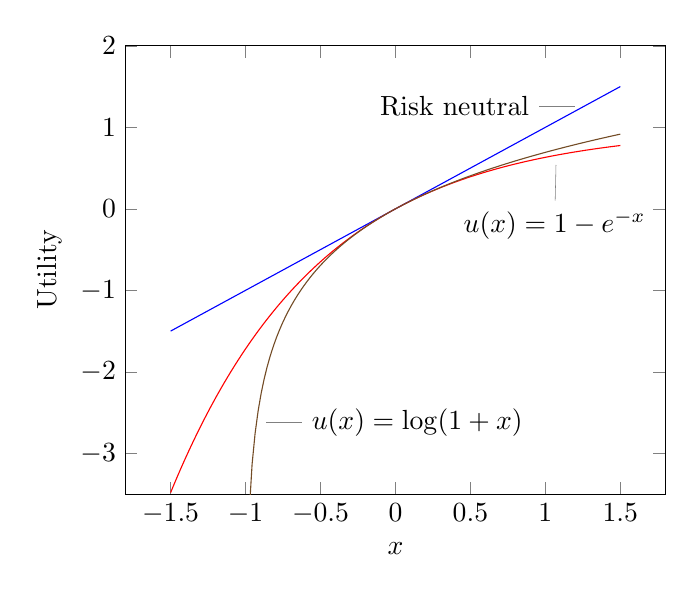
\begin{tikzpicture}
      \begin{axis}[
        xlabel=$x$,
        ylabel=Utility,
        domain=-1.5:1.5,
        samples=150,
        ymin=-3.5
        ]
        \addplot+[mark=none] {x}
        node[pos=0.92, pin={[black]180:Risk neutral}]{};
        \addplot+[mark=none] {1-exp(-x)}
        node[pos=0.92, pin={[black]-92:$u(x)=1-e^{-x}$}] {};
        \addplot+[mark=none] {ln(1+x)}
        node[pos=0.4, pin={[black]0:$u(x)=\log(1+x)$}] {};
      \end{axis}
    \end{tikzpicture}
    \caption{Comparison of the exponential and logarithmic
      utilities. As $x$ approaches -1 from above, the utility to a logarithmic
      decision maker is modelled to be infinitely bad.
    }\label{fig:example_utilities}
  \end{figure}
\end{example}

For a given utility function that models a decision maker's measure of
benefit for the outcomes of $f$, one can define an ordering
between random variables that decides which of any two decisions
$x_1,x_2\in\mathcal{X}$ is better.
\begin{mydef}[Expected utility ordering]
  A utility function $u(x)$ defines an ordering $\preceq$ between random
  variables $X$ and $Y$,
  \begin{equation}
    X\preceq Y \Leftrightarrow \mathbb E[u(X)] \leq \mathbb E[u(Y)].
  \end{equation}
\end{mydef}

We can therefore formulate a well-defined optimisation problem by
modelling the decision maker's attitude to risk with utility functions.

\begin{problem}[Expected utility]
  The optimal choice to maximise a given utility of $f$ is the
  solution of
  \begin{align}
    x(u)=\argmax_{x\in\mathcal{X}} \mathbb E[u(f(x,\cdot))].
  \end{align}
\end{problem}


\subsection{Mean-deviation problems}
The expected utility approach considers the mean outcome of a choice.
After one makes a decision $x\in\mathcal{X}$, the realisation of the
parameter in $\mathcal{Y}$ only happens once. If there is a large
uncertainty in $f(x,\cdot)$, the average value may not be a good
representation for the realised value of $f$.
It can therefore be useful to take into account some measure of
deviation from the mean of $f$ when $x$ is chosen.
The mean-deviation approach aims to balance the expected value of $f$
with uncertainty represented by a deviation measure.
\begin{mydef}[Deviation measure]
  A functional $\mathbb D$ on a linear space of random
  variables containing the real numbers defines a deviation measure, if:
  \begin{enumerate}
  \item $\mathbb D[C] = 0$ for any constant $C$,
  \item $\mathbb D[X]>0$ for non-constant random variables $X$.
  \end{enumerate}
  This work will mainly consider convex deviation measures.
\end{mydef}

\begin{example}[Deviation measures]
  The classic measure of deviation is the standard deviation, which is
  a particular case of the deviation measures defined by
  the $L^p$-norms:
  \begin{align}
    X\mapsto \|X-\mathbb EX\|_p,\; p\geq 1.
    && \text{($L^p$-deviations)}
  \end{align}

  In a maximisation setting, one might not be worried about
  realisations of $f$ that are larger than its mean, especially if the
  random variable is not symmetric.
  The lower semi-deviation measure only investigates
  worse-than-expected outcomes:
  \begin{align}
    X\mapsto \mathbb E[\max(\mathbb E[X]-X,0)].
    &&\text{(Lower semi-deviation)}
  \end{align}

  One can also combine two deviation-measures in order to capture
  different aspects of a random variable.
  If $\mathbb D_1,\dots,\mathbb D_k$ are $k$ deviation measures and
  $\lambda_i>0$, then the following is also
  is also a deviation measure:
  \begin{align}
    \mathbb D[X]=\sum_{i=1}^k\lambda_i\mathbb D[X].
    &&\text{(Weighted deviations)}
  \end{align}

  If $\mathbb U$ is a nonlinear expectation from
  \Cref{sec:nonlinear_expectations} with $\mathbb U[X]< \mathbb
  E[X]$ for all non-constant $X$,
  then one can
  construct a deviation measure with the functional
  $\mathbb D[X]=\mathbb E[X]-\mathbb U[X]$.
  This is equal to $X\mapsto -\mathbb U[X-\mathbb E[X]]$ in all the
  examples given below.
\end{example}

For a given deviation measure that models the decision maker's
need for stability, one can formulate a bi-objective optimisation
problem.
\begin{problem}[Mean-deviation]
  An optimal decision that maximises the expected value of $f$ whilst
  minimising the deviation $\mathbb D$ of $f$, is a minimiser to the
  bi-objective optimisation problem
  \begin{align}
    \min_{x\in\mathcal{X}}\{(-\mathbb E[f(x,\cdot)],\,\mathbb D[f(x,\cdot)])\}.
  \end{align}
\end{problem}
We can approach the bi-objective problem from a multiobjective
optimisation theory point of view, and will do so in
\Cref{sec:one_multiobjective}.
The review in \citep{marler2004survey} covers some of the theory,
discusses what optimality means and introduces approaches to solve them.
A simple approach is to define a single objective function that combines
the expected value with a deviation-penalty, weighted by some
parameter $\lambda>0$. The optimal decision in $\mathcal{X}$ is then
defined as
\begin{equation}\label{eq:mean_dev_weighted}
  x(\mathbb D,\lambda)=\argmax_{x\in\mathcal{X}}\{\mathbb
  E[f(x,\cdot)]-\lambda \mathbb D[f(x,\cdot)]\}.
\end{equation}
This implicitly defines an ordering of random variables based on
the functional $X\mapsto \mathbb{E}[X]-\lambda \mathbb{D}[X]$.
If $f$ is nonlinear, then $x(\mathbb D,\lambda)$ can be unstable to
small changes in $\lambda$. Small errors in determining the best
$\lambda$ to represent a decision-maker can cause large changes in
either of the objectives. The review \citep{marler2004survey} covers
more robust methods.

\subsection{Nonlinear expectations}\label{sec:nonlinear_expectations}
A general framework that covers most of the remaining
in optimisation under uncertainty makes use of a class of functionals
called nonlinear expectations.
The theory was developed in finance to study financial positions using
risk measures, see
e.g.~\citep[Ch.~4]{follmer2004stochastic}.
Risk measures are used in a minimisation setting related to losses,
and we will use the term nonlinear expectations in the maximisation
setting. The examples of nonlinear expectations $\mathbb U$ considered
in this section give rise to well-known risk measures $\rho$, by using the mapping
$\rho(X) = -\mathbb U[X]$.

\begin{mydef}[Nonlinear expectation]
  A nonlinear expectation $\mathbb U$ is a functional on a linear space of random
  variables containing the real numbers, such that:
  \begin{enumerate}
  \item $\mathbb U[C] = C$ for any constant $C$,
  \item $\mathbb U[X]\leq \mathbb U[Y]$ whenever $X\leq Y$ almost surely.
  \end{enumerate}
  This work will mainly consider concave nonlinear expectations, that
  is, nonlinear expectations $\mathbb{U}$ such that
  $\mathbb{U}[\lambda X + (1-\lambda)Y]\geq \lambda\mathbb{U}[X] +
  (1-\lambda) \mathbb{U}[Y]$ for any $\lambda\in[0,1]$ and random
  variables $X,Y$.
\end{mydef}

\begin{example}[Nonlinear expectations]
  The functional $\mathbb U_\lambda[X]=-\frac{1}{\lambda}\log\mathbb
  E[e^{-\lambda X}]$, is called the entropic nonlinear expectation,
  with $\lambda>0$.
  It is connected to the exponential utility function $u_\lambda$, since
  $\mathbb U_\lambda[X]= u_\lambda^{-1}(\mathbb E[u_\lambda(X)])$.

  The worst-case nonlinear expectation on the sample space $\Omega$,
  defined by
  $X\mapsto  \inf_{\omega\in\Omega}X(\omega)$, connects this theory with robust
  programming. If there is an attached probability space on $\Omega$,
  we use the essential infimum.

  For some deviation measures $\mathbb D$, such as the lower
  semi-deviation, the functional $\mathbb U(X)=\mathbb E[X]-\mathbb
  D[X]$ defines a nonlinear expectation. Note that for a general space
  of random variables the symmetric deviation measure, such as the
  standard deviation, do not give rise to a nonlinear
  expectation: They can violate the monotonicity requirement.

  The quantile operator
  $q_\lambda[X] = \inf\{x\mid\mathbb P(X\leq x)>
  \lambda\}$ satisfies the properties of a nonlinear expectation.
  Note that the operator is not necessarily concave, which has
  implications for the resulting optimisation problem.
  A concave lower bound on the quantile operator is
  the lower super-quantile.
  \begin{equation}\label{eq:def_avar}
    \mathbb U_\lambda[X]=\frac{1}{\lambda}\int_0^\lambda q_t[X]\,\dt.
  \end{equation}
  Another name for the quantile operator is Value at Risk.
  The risk measures related to the lower super-quantile operator are also referred to as
  the Expected Shortfall, Average Value at Risk, and Conditional Value at Risk.
  \citep{artzner1999coherent,rockafellar2002conditional,follmer2004stochastic}.
  Their definitions all coincide with~\eqref{eq:def_avar} when the
  cumulative distribution function of $X$ is continuous, however, in
  the general case they handle discontinuities differently.
\end{example}

\begin{problem}[Nonlinear expectation]
  The optimal choice to maximise a nonlinear expectation
  of $f$ is given by
  \begin{align}
    x(\mathbb U)=\argmax_{x\in\mathcal{X}} \mathbb U[f(x,\cdot)].
  \end{align}
\end{problem}

Note that the solutions of the nonlinear expectation and expected
utility problems coincide if one uses the entropic measure and the exponential
utility respectively.
\begin{example}[Lower super-quantile]
  Following \citep{ben2007old}, we can reformulate the lower
  super-quantile optimisation problem arising from~\eqref{eq:def_avar}
  by introducing an auxiliary variable $\eta\in\mathbb R$.
  \begin{equation}\label{eq:opt_avar}
    x_{sq}({\gamma})
    =\argmax_{x\in\mathcal X,\eta\in\mathbb R}
    \{\eta - \frac{1}{\gamma}\mathbb E[\max(\eta-f(x,\cdot),0)]\}.
  \end{equation}
  Note that the objective is not necessarily smooth, due to the
  $\max(\eta-f(x,\cdot),0)$ term. Theory of non-smooth optimisation
  can address this, but may require heavy mathematical machinery, as
  exemplified in~\cite{kouri2016risk}.
\end{example}


\section{Different approaches lead to the same decision}\label{sec:one_comparison_orderings}
The aim of this section is to compare the
optimisation formulations introduced in the previous section.
Can the mean-deviation formulation give the
same result as the expected utility and nonlinear expectation methods?
If $f(x,\cdot)$ is normally distributed for each value of
$x\in\mathcal{X}$, then the properties of the random variable is fully
described by the mean and variance functions $x\mapsto
\mathbb{E}[f(x,\cdot)]$ and $x\mapsto \mbox{Var}[f(x,\cdot)]$. This
indicates that all the approaches above implicitly define a
choice of ordering for the bi-objective mean-standard deviation
optimisation problem.

\begin{example}[Lower super-quantile]\label{ex:avar_normal}
  Let $X=\mathbb{E}[X]+ \sqrt{\mbox{Var}[X]} Z$ for $Z\sim\mathcal{N}(0,1)$.
  Then the $\gamma$-quantile of $X$ is
  $q_\gamma[X] = \mathbb{E}[X] + \sqrt{\mbox{Var}[X]} q_\gamma[Z]$.
  Thus, the lower super-quantile $\mathbb{U}_\gamma$ of $X$ depends only on
  its mean and variance, with
  \begin{equation}
    \mathbb{U}_\gamma[X] =  \mathbb{E}[X]
    + \sqrt{\mbox{Var}[X]} \mathbb{U}_\gamma[Z].
  \end{equation}
  Note that $\mathbb{U}_\gamma[Z]\leq 0$ for each $\gamma\in[0,1]$,
  with equality only when $\gamma=1$.
  The lower super-quantile optimisation problem is therefore
  a special case of the mean-deviation optimisation problem
  with $\mathbb{D}[X]=\sqrt{\mbox{Var}[X]}$,
  using the weighted sum ordering from~\eqref{eq:mean_dev_weighted} and
  $\lambda = -\mathbb{U}_\gamma[Z]$.
\end{example}

\begin{example}[Exponential utility]
  Let $X=\mathbb{E}[X]+ \mathbb{D}[X] Z$, as in \Cref{ex:avar_normal}.
  Then its exponential utility $u$ with parameter $\mu$
  is
  \begin{equation}
    u(X) = 1 - e^{-\mu (\mathbb{E}[X] +
      \mathbb{D}[X] Z)}.
  \end{equation}
  If $f(x,\cdot)$ is normally distributed, the expected utility
  optimisation for $u$ is then equivalent to solving
  \begin{equation}
    \min_{x\in\mathcal{X}}  e^{-\mu\mathbb{E}[f(x,\cdot)]}
    \mathbb{E} \left[ e^{-\mu \mathbb{D}[f(x,\cdot)] Z} \right].
  \end{equation}
  In the context of multiobjective optimisation, this is equivalent to
  a particular choice of ordering of the mean-standard deviation problem.
\end{example}

The review \citep{nadarajah2014estimation} of estimation methods for
lower super-quantiles provide further evidence that people use
the first two moments of a random variable to estimate nonlinear
expectations for more generic distributions.

Consider now the decisions that arise from the following
optimisation problems of mean-deviation, exponential utility, and
lower super-quantile $\mathbb{U}_\gamma$.
\begin{subequations}\label{eq:optim_formulations}
  \begin{align}
    x_{md}(\lambda)
    &=\argmax_{x\in\mathcal X}\{\mathbb
      E[f(x,\cdot)]-\lambda\sqrt{\mbox{Var}[f(x,\cdot)]}\}
    &\lambda\geq 0,\\
    % &&\text{(mean-deviation)},\\
    x_{eu}(\mu)
    &=\argmax_{x\in\mathcal X}\{
      \mathbb E[1-e^{-\mu f(x,\cdot)}]\}
    &\mu>0,\\
    % &&\text{(exponential utility)},\\
    x_{sq}(\gamma)
    &=\argmax_{x\in\mathcal X}
      \{\mathbb U_\gamma[f(x,\cdot)]\}
    &\gamma\in(0,1].
    % &&\text{(lower super-quantile)}.
  \end{align}
\end{subequations}
One may ask if there are triples of $(\lambda,\mu,\gamma)$ that give rise
to the same decisions, $x_{md}=x_{eu}=x_{sq}$?
We can investigate this question in the following way.
For a given value $\mu>0$ or $\gamma\in(0,1]$, find the minimisers
$\lambda(\mu)$ and $\lambda(\gamma)$ of

\begin{subequations}\label{eq:min_xmd_xeu_xsq}
  \begin{align}
    \label{eq:min_xmd_xeu}
    &\min_{\lambda\geq 0}\{{\|x_{md}(\lambda)-x_{eu}(\mu)\|}_2\},
      \textnormal{ and}\\
    &\min_{\lambda\geq 0}\{{\|x_{md}(\lambda)-x_{sq}(\gamma)\|}_2\}.
  \end{align}
\end{subequations}
If the minimum is close to zero, it is an indication that either method
can be used to model the risk-preferences of a particular decision maker.
\Cref{fig:util_meandev_2d} shows the result of such an investigation,
and for the particular example considered the differences are small.
In general, it is likely to be examples where the choice of
optimisation formulation matters for the decision. The purpose of this
section is to highlight that one should investigate the structure of
a problem and choose among the computationally tractable options based
on their practical implications instead of solely focusing on
theoretical properties of the different formulations.

\begin{example}[Pricing problem]
  Let us consider a particular decision problem and compare the
  decisions of~\eqref{eq:optim_formulations}.
  We must choose the prices $x_1$, $x_2$ of two products in order to
  maximise the total profit for some time period.
  Assume that the model for product demand $q=(q_1,q_2)$ for the two products in
  this period is
  deterministic and defined by the functions
  \begin{align}
    q_1(x) &= e^{-2x_1}(1-e^{-10x_2}),
    &q_2(x)&= 0.9e^{-1.8x_1}(1-e^{-4x_2})
  \end{align}
  respectively.
  The term $e^{-2x_1}$  models the impact of price
  changes for product one, keeping product two's price constant.
  The term $1-e^{-10x_2}$ models the proportion of product one's
  demand that product two takes at price $x_2$.
  \Cref{fig:total_volume_2d} shows the total demand $q_1+q_2$.
  \begin{figure}[htbp]
    \centering
    \includegraphics{total_volume_2d}
    \caption{The sum $q_1+q_2$ shows the total demand for the two products.
      Note that in the retail setting, the values near $x=(0,0)$ seem
      nonsensical.}\label{fig:total_volume_2d}
    \todo[inline]{Update plot}
  \end{figure}

  Given unit costs $y=(y_1,y_2)$, the profit $f(x,y)$ is then
  \begin{align}
    f(x)
    &=\langle x-y,q(x) \rangle,
    &\langle \cdot,\cdot \rangle
      \textnormal{ is the inner product on } \mathbb{R}^n.
  \end{align}
  Retailers often face uncertain unit costs for their products, which
  we model with a random variable $y\in\mathbb{R}^2$.
  Denote the mean and covariance of
  $y$ by $m_y$ and $C_y$ respectively. Then
  \begin{align}
    \mathbb{E}[f(x,y)]
    &= \langle x-m_y,v(x) \rangle,
    &\mbox{Var}[f(x,y)]
    &= \langle v(x),C_y v(x) \rangle.
  \end{align}
  Thus, the mean-deviation method with
  $\mathbb{D}[X]=\sqrt{\mbox{Var}[X]}$ has a closed form objective and
  one only needs information about the two first moments of $y$ to perform
  the optimisation.

  For this particular example we model the unit costs $y$ as a log-normally
  distributed random variable with mean and covariance
  \begin{align}
    m_y
    &= (0.5,0.5),
    &C_y
    &=\begin{pmatrix}
      2.5&-0.75\\
      -0.75&2.5
    \end{pmatrix}
             \times 10^{-3}.
  \end{align}

  We solve the optimisation problems in~\eqref{eq:min_xmd_xeu_xsq}
  uniformly spaced values $\mu\in[0,100]$ and $\gamma\in[1/100, 1]$.
  \Cref{fig:util_meandev_2d,fig:cvar_meandev_2d} show the
  corresponding values $\lambda(\mu)$ and $\lambda(\gamma)$, together
  with the difference in the objectives. The values of $\lambda$
  are stable to small changes in $\mu$ and $\gamma$, and the
  price differences are unlikely to have a practical effect when
  priced in-store.
  \begin{figure}[htbp]
    \centering
    \includegraphics[width=\textwidth]{util_meandev_2d}
    \caption{The right plot shows the $\ell_2$-norm difference between the decision made
      from the mean-deviation and exponential utility methods defined in
      \Cref{eq:optim_formulations}, using the corresponding
      $(\mu,\lambda)$-pairs from the left plot.
    }\label{fig:util_meandev_2d}
    \todo[inline]{update plot}
  \end{figure}

  \begin{figure}[hbtp]
    \centering
    \includegraphics[width=\textwidth]{cvar_meandev_2d}
    \caption{The right plot shows the $\ell_2$-norm difference between the decision made
      from the mean-deviation and super-quantile methods defined in
      \Cref{eq:optim_formulations}, using the corresponding
      $(\gamma,\lambda)$-pairs from the left plot.
    }\label{fig:cvar_meandev_2d}
    \todo[inline]{update plot}
  \end{figure}
\end{example}

\subsection{Discussion}
The use of super-quantiles in revenue management has become popular
the last ten years
\citep{wu2014risk,xue2015optimal,zhou2008optimal,ahmed2007coherent}.
These articles argue for super-quantiles and dismiss
optimisation formulations that use the mean and standard deviation
on the grounds that they penalise better-than-expected outcomes.
Distributions of profit in revenue management do in practice, however,
have a more significant lower tail than upper tail, due to inventory
restrictions, which alleviates such problems.
None of these references discuss to what extent super-quantiles change the
optimal decisions for their presented problems compared to a
mean-deviation approach.
The authors of \citep{choi2011multiproduct}
dismiss the mean-deviation
problem by formulating it in terms of the weighted sum of mean and
variance, and then argue that the units of these objects do not
coincide.

The exponential utility and lower super-quantile are often more costly
to compute or approximate than the mean and variance, and requires a
full description of the distribution of $y$. If, for a given $\mu$ (or
$\gamma$), it is possible to find a $\lambda$ such that
$x_{md}(\lambda)$ is close to $x_{eu}(\mu)$ (or $x_{sq}(\gamma)$), then the
mean-deviation formulation may be preferable in practical settings.
Two articles illustrating this are
\citep{kouri2016risk,alexanderian2017mean}, who address optimisation problems
where each value $y\in\mathcal{Y}$ require the solution to partial
differential equations.
For example,~\cite{kouri2016risk}
need to draw samples from $\mathcal{Y}$ and find ways to smooth the lower super-quantile,
whilst~\cite{alexanderian2017mean} approximate mean and variance
with Taylor series and do not need to sample from $\mathcal{Y}$.


\section{Randomness and constraints}
Let us introduce another, deterministic, objective $g:\mathcal
X\to\mathbb R$. In the deterministic setting, with a known parameter
$y\in\mathcal{Y}$, one often considers problems of the form
\begin{align}
  \min_{x\in\mathcal{X}}\{g(x)\mid f(x,y)\geq f_{\textnormal{min}} \},\;
  \text{ for some } f_{\textnormal{min}}\in\mathbb R.
\end{align}
Then $f\geq f_{\textnormal{min}}$ is considered a constraint, which restricts the
decision space to $\{x\in\mathcal{X}\mid f(x,y)\geq f_{\textnormal{min}}\}$.
When there is uncertainty about the right parameter-value, this set is
not defined at the time of decision, but depends on future knowledge
of the parameter.

In the engineering community it is popular to
reinterpret non-deterministic ``constraints'' as deterministic via
expected utilities, mean-deviation methods or nonlinear
expectations
\citep{rockafellar2007coherent,rockafellar2015engineering}.
Such a reinterpretation defines an acceptance set $\mathcal{A}$ that
tries to represent what a decision maker deems to be feasible in a
risk-adjusted way, and results in the optimisation problem
$\min_{x\in\mathcal{A}} g(x)$.
The acceptance set approach was one of the motivations for a formal
framework for risk measures, in introduced in \citep{artzner1999coherent}.
\begin{example}[Acceptance sets]
  Popular choices of acceptance sets for the constraint $f(x,y)\geq
  f_{\textnormal{min}}$ are
  \begin{align}
    \mathcal{A}&=\{x\in\mathcal X \mid
                 \mathbb E_y[f(x,y)]\geq f_{\textnormal{min}}\}, \\
    \mathcal{A}&=\{x\in\mathcal X \mid
                 \inf_{\omega\in\Omega}f(x,y(\omega))\geq f_{\textnormal{min}}\},\\
    \mathcal{A} &= \{x\in\mathcal X\mid
                  \mathbb P_y(f(x,y)\geq f_{\textnormal{min}})\geq \epsilon\},
                  \text{ given }\epsilon\in(0,1).
  \end{align}
\end{example}

The acceptance set approach treats what was previously considered a
hard constraint in terms of marginalised values that allow decisions $x\in\mathcal{X}$
that may violate the originally intended constraint for some values of the random
variable $y$. We believe that a better approach is to take one step back
and model the trade-off between $g(x)$ and the outcomes of $f(x,y)$,
which is a multiobjective optimisation approach.

\section{Multiobjective optimisation}\label{sec:one_multiobjective}

\begin{itemize}
\item Copy stuff from transfer thesis
\item Include (and update) MultiJuMP example
\item Show example of mean-std with revenue: Pareto is not convex
\end{itemize}

\todo[inline]{Say that optimisation with random outcomes is a possibly
  infinite-number-of-objectives problem}




\biblio{} % Bibliography when standalone
\end{document}

%%% Local Variables:
%%% mode: latex
%%% TeX-master: t
%%% TeX-command-extra-options: "--shell-escape"
%%% TeX-command-extra-options: "-shell-escape"
%%% End:
